%% Type de document et encodage de la police
\documentclass[a4paper]{article}
\usepackage[utf8x]{inputenc}
\usepackage[T1]{fontenc}
\usepackage[colorlinks=true, allcolors=black]{hyperref}
% \usepackage[french]{babel}

%% Initialise la taille des pages et des marges
\usepackage[a4paper, top=3cm, bottom=3cm, left=2cm, right=2cm, marginparwidth=2cm]{geometry}

%% Packs utiles
\usepackage{amsmath}
\usepackage{graphicx}
\usepackage{xcolor}
\usepackage{multirow}

%% Commandes perso
\renewcommand{\arraystretch}{1.2} %% row 20% longer
\renewcommand{\contentsname}{Table des matières}
\definecolor{sprinen}{rgb}{0.0, 1.0, 0.7}
\renewcommand\labelitemi{--}

%% Pour les exemples
\usepackage{mdframed}
\newmdenv[topline=false, bottomline=false, rightline=false, skipabove=\topsep, skipbelow=\topsep]{example}

%% Pour les diagrammes
\usepackage{tikz}
\usetikzlibrary{shapes}
\tikzstyle{incolore} = [rectangle, draw=black, minimum height=1cm, minimum width=3cm, text width=3cm, text centered, anchor=north west]
\tikzstyle{choice} = [diamond, text width=2cm, text centered, fill=blue!30, rounded corners]


\title{Sécurité des réseaux : Netfilter \& Palo Alto}
\author{Grégoire Roumache}
\date{Avril 2021}

\begin{document}

\maketitle















\section{Netfilter}





\begin{center} 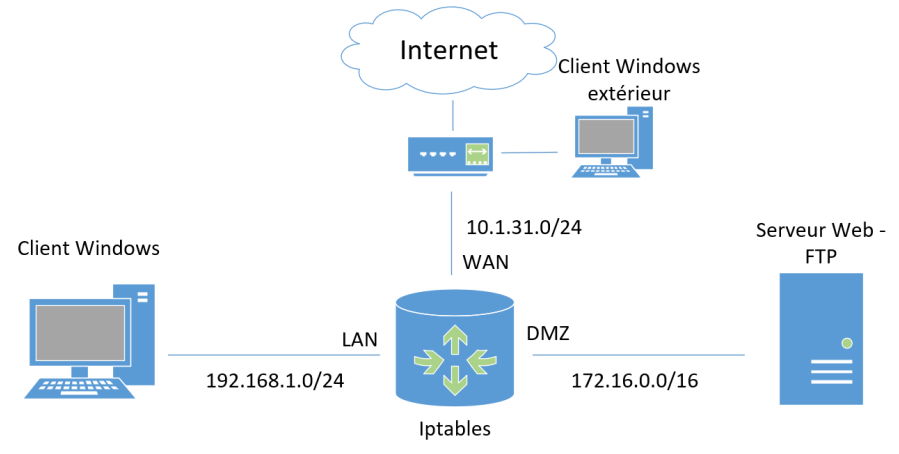
\includegraphics[width=0.95\linewidth]{images/topologie-netfilter-01.PNG} \end{center}


\begin{itemize}


\item Configurations réseaux (dns = 208.67.222.123 - opendns):
\begin{enumerate}
    \item Windows (réseau interne - lan):
    \begin{center} \begin{tabular}{|c|c|} \hline
        ip      & 192.168.1.2   \\ \hline
        netmask & 255.255.255.0 \\ \hline
        gateway & 192.168.1.1   \\ \hline
    \end{tabular} \end{center}
    \item Serveur (réseau interne - dmz):
    \begin{center} \begin{tabular}{|c|c|} \hline
        ip      & 172.16.0.2  \\ \hline
        netmask & 255.255.0.0 \\ \hline
        gateway & 172.16.0.1  \\ \hline
    \end{tabular} \end{center}
    \item Firewall:
    \begin{center} 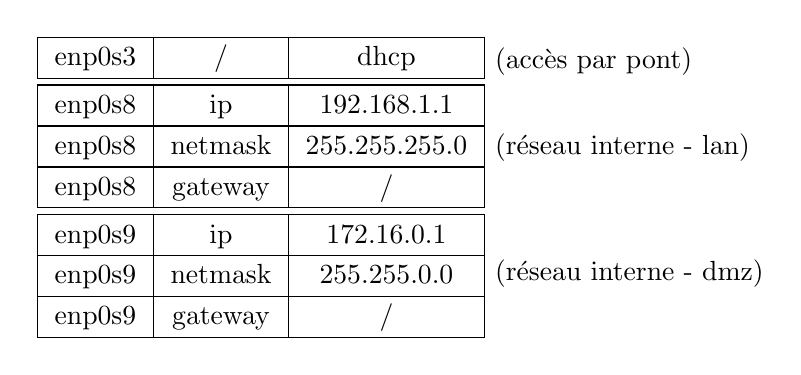
\begin{tikzpicture}
        \node () [] at (0,0)
            {\begin{tabular}{|c|c|c|} \hline
                enp0s3 & /       & dhcp
                \\ \hline \hline
                enp0s8 & ip      & 192.168.1.1   \\ \hline
                enp0s8 & netmask & 255.255.255.0 \\ \hline
                enp0s8 & gateway & /
                \\ \hline \hline
                enp0s9 & ip      & 172.16.0.1  \\ \hline
                enp0s9 & netmask & 255.255.0.0 \\ \hline
                enp0s9 & gateway & /  \\ \hline
            \end{tabular}};
        \node () [anchor=west] at (2.85,+1.6) {(accès par pont)};
        \node () [anchor=west] at (2.85,+0.5) {(réseau interne - lan)};
        \node () [anchor=west] at (2.85,-1.1) {(réseau interne - dmz)};
    \end{tikzpicture} \end{center}
\end{enumerate}


\begin{center} 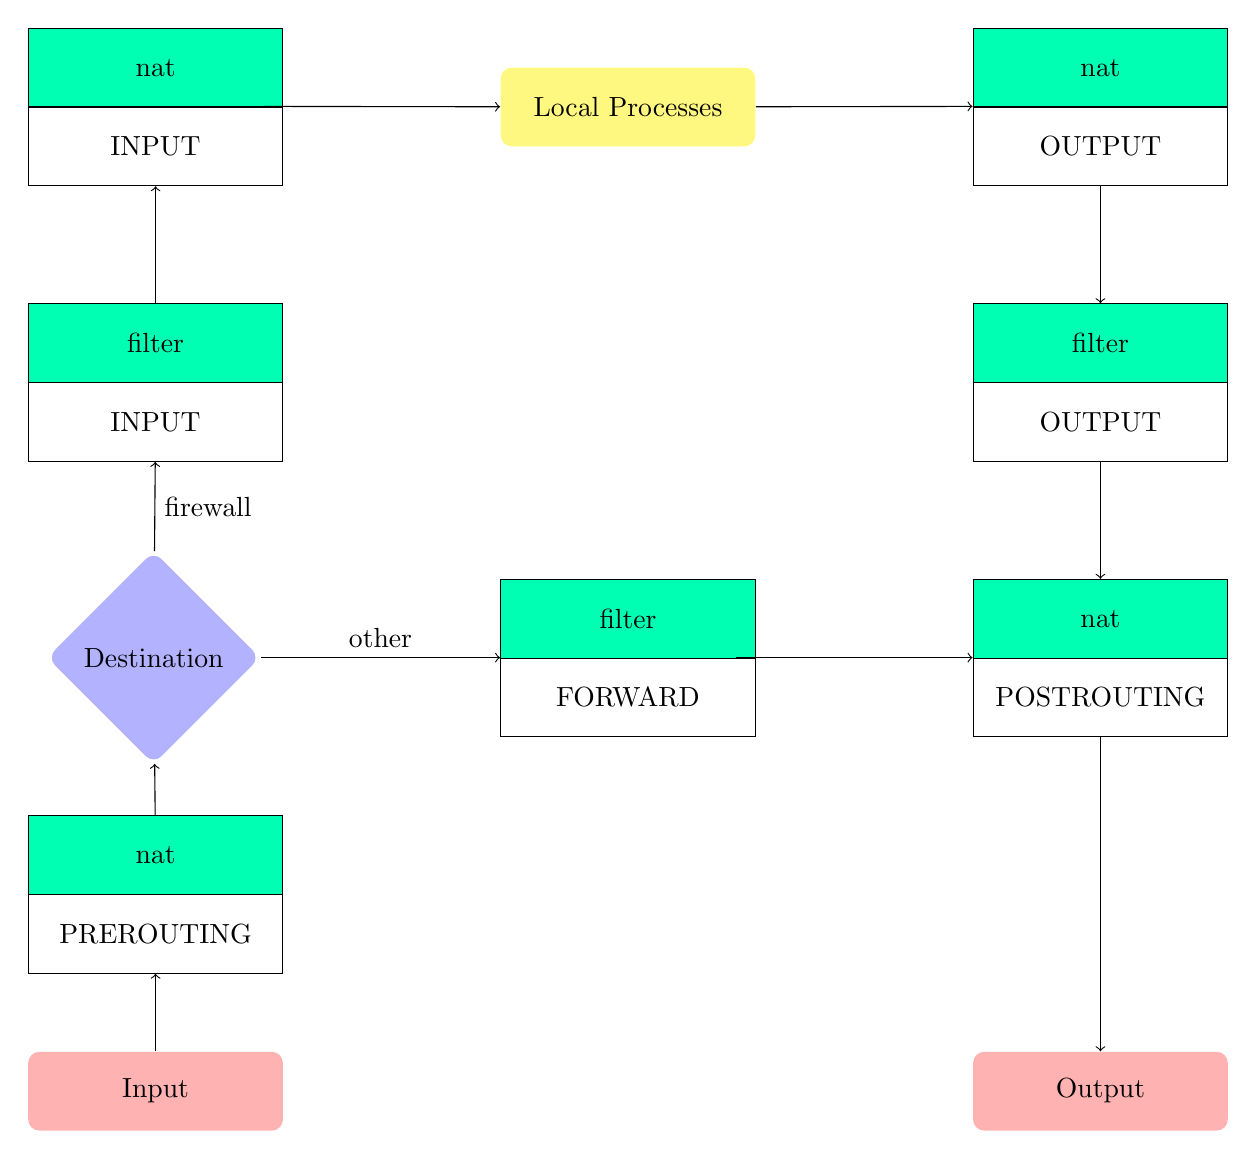
\begin{tikzpicture}

    \node (natPreroutingUp) [incolore, fill=sprinen] at (0,0) {nat};
    \node (natPreroutingDown) [incolore] at (0,-1) {PREROUTING};

    \node (natInputUp) [incolore, fill=sprinen] at (0,10) {nat};
    \node (natInputDown) [incolore] at (0,9) {INPUT};

    \node (filterInputUp) [incolore, fill=sprinen] at (0,6.5) {filter};
    \node (filterInputDown) [incolore] at (0,5.5) {INPUT};

    \node (natOutputUp) [incolore, fill=sprinen] at (12,10) {nat};
    \node (natOutputDown) [incolore] at (12,9) {OUTPUT};

    \node (filterOutputUp) [incolore, fill=sprinen] at (12,6.5) {filter};
    \node (filterOutputDown) [incolore] at (12,5.5) {OUTPUT};

    \node (natPostroutingUp) [incolore, fill=sprinen] at (12,3) {nat};
    \node (natPostroutingDown) [incolore] at (12,2) {POSTROUTING};

    \node (filterForwardUp) [incolore, fill=sprinen] at (6,3) {filter};
    \node (filterForwardDown) [incolore] at (6,2) {FORWARD};

    \node (WAN) [incolore, rounded corners, fill=red!30, draw=none] at (0,-3) {Input};
    \node (LAN) [incolore, rounded corners, fill=red!30, draw=none] at (12,-3) {Output};

    \node (firewall) [incolore, rounded corners, fill=yellow!50, draw=none] at (6,9.5) {Local Processes};
    \node (forward) [choice, xshift=0.1cm] at (1.5,2) {Destination};

    \draw[->] (WAN) -- (natPreroutingDown);
    \draw[->] (natPreroutingUp) -- (forward);
    \draw[->] (forward) -- node[anchor=west]{firewall} (filterInputDown);
    \draw[->] (forward) -- node[anchor=south]{other} (6,2);
    \draw[->] (3,9) -- (firewall);
    \draw[->] (firewall) -- (12,9);
    \draw[->] (natOutputDown) -- (filterOutputUp);
    \draw[->] (filterOutputDown) -- (natPostroutingUp);
    \draw[->] (9,2) -- (12,2);
    \draw[->] (natPostroutingDown) -- (LAN);
    \draw[->] (filterInputUp) -- (natInputDown);

\end{tikzpicture} \end{center}


\item Tables et chaines:
\begin{enumerate}
    \item Filter
    \begin{itemize}
        \item input/ouput = paquets en provenance/destination du parefeu
        \item forward = paquets traversant le parefeu
    \end{itemize}
    \item Nat
    \begin{itemize}
        \item input/ouput = paquets en provenance/destination du parefeu
        \item prerouting/postrouting = modification des ip dans les paquets pour le nat
    \end{itemize}
\end{enumerate}


\item Tableau de règles (table nat):
\begin{center} \begin{tabular}{|c|c|c|c|c|c|c|c|} \hline

    \textbf{chain} & \textbf{type} & \textbf{input} & \textbf{output} & \textbf{input} & \textbf{output} & \textbf{protocole} & \textbf{port} \\
    && \textbf{interface} & \textbf{interface} & \textbf{ip} & \textbf{ip} &&
    \\ \hline \hline

    postrouting & snat & \texttt{<lan>} & \texttt{<wan>} & \texttt{<wan>} & / & / & / \\ \hline
    postrouting & snat & \texttt{<dmz>} & \texttt{<wan>} & \texttt{<wan>} & / & / & /
    \\ \hline \hline

    prerouting & dnat & \texttt{<wan>} & \texttt{<dmz>} & / & \texttt{<dmz>} & tcp & 20,21,80 \\ \hline
    prerouting & dnat & \texttt{<wan>} & \texttt{<dmz>} & / & \texttt{<dmz>} & tcp & 61337:22 \\ \hline

\end{tabular} \end{center}


\newpage


\item Tableau de règles (table filter):
\begin{center} \begin{tabular}{|c|c|c|c|c|c|c|c|c|} \hline

    \textbf{chain} & \textbf{priority} &
    \textbf{source} & \textbf{source} & \textbf{dest.} & \textbf{dest.} &
    \textbf{protocol} & \textbf{ouput} & \textbf{permission} \\

    && \textbf{ip} & \textbf{port} & \textbf{ip} & \textbf{port} &
    & \textbf{interface} & \\ \hline \hline

    %%%%%%%%%%%%%%% tout interdire %%%%%%%%%%%%%%%

    input & 999 &
    * & * & * & * &
    * & * & reject \\ \hline

    output & 999 &
    * & * & * & * &
    * & * & reject \\ \hline

    forward & 999 &
    * & * & * & * &
    * & * & reject \\ \hline \hline

    %%%%%%%%%%%%%%% tout autoriser sur l'interface loopback %%%%%%%%%%%%%%%

    input & 1 &
    * & * & * & * &
    * & lo & accept \\ \hline

    output & 1 &
    * & * & * & * &
    * & lo & accept \\ \hline \hline

    %%%%%%%%%%%%%%% LAN -> WAN %%%%%%%%%%%%%%%

    forward & 1 &
    \texttt{<lan>} & * & * & 443 &
    tcp & \texttt{<wan>} & accept \\ \hline

    forward & 1 &
    \texttt{<lan>} & * & \texttt{<dns>} & 53 &
    udp & \texttt{<wan>} & accept \\ \hline \hline

    %%%%%%%%%%%%%%% LAN -> DMZ %%%%%%%%%%%%%%%

    forward & 1 &
    \texttt{<lan>} & * & * & * &
    icmp & \texttt{<dmz>} & accept \\ \hline

    forward & 1 &
    \texttt{<lan>} & * & * & 20,21,80 &
    tcp & \texttt{<dmz>} & accept \\ \hline \hline

    %%%%%%%%%%%%%%% WAN -> DMZ %%%%%%%%%%%%%%%

    forward & 1 &
    \texttt{<wan>} & * & * & 20,21,80 &
    tcp & \texttt{<dmz>} & accept \\ \hline

    forward & 1 &
    \texttt{<wan>} & * & * & 22 &
    tcp & \texttt{<dmz>} & accept \\ \hline \hline

    %%%%%%%%%%%%%%% ANY -> Firewall %%%%%%%%%%%%%%%

    input & 1 &
    \texttt{<wan>} & * & \texttt{<firewall>} & * &
    icmp & / & accept \\ \hline

    input & 1 &
    \texttt{<lan>} & * & \texttt{<firewall>} & * &
    icmp & / & accept \\ \hline

    input & 1 &
    \texttt{<dmz>} & * & \texttt{<firewall>} & * &
    icmp & / & accept \\ \hline \hline

    %%%%%%%%%%%%%%% Client externe -> Firewall %%%%%%%%%%%%%%%

    input & 1 &
    \texttt{<wan>} & * & \texttt{<firewall>} & 22 &
    tcp & / & accept \\ \hline

\end{tabular} \end{center}
\textbf{Remarque}: on n'autorise pas le protocole https directement mais le protocole tcp et le port 443 car le contenu est chiffré.


\item Afficher les règles iptables:
\begin{example}
    \begin{itemize}
        \item \texttt{iptables -t filter -L [<chaine>] -{}-line-numbers -n}
        \item \texttt{iptables -t nat -L [<chaine>] -{}-line-numbers -n}
    \end{itemize}
\end{example}
\textbf{Remarque}: dès qu'un paquet correspond à une règle, cette règle s'applique et les autres sont ignorées.


\item Pour transformer la machine debian en routeur, il faut décommenter la ligne suivante dans \texttt{/etc/sysctl.conf}:
\begin{example} \begin{verbatim}
net.ipv4.ip_forward=1
\end{verbatim} \end{example}
\textbf{Remarque}: il faut ajouter des default gateways sur toutes les machines (sauf si dhcp).


\item Utiliser conntrack pour permettre le trafic provenant de connexions déjà établies:
\begin{example} \begin{itemize}
    \item Installer conntrack: \texttt{apt install conntrack}
    \item Lister les connexions: \texttt{conntrack -L}
    \item Autoriser les connexions établies/liées:
    \begin{example}
        \texttt{iptables -A INPUT -m conntrack -{}-ctstate ESTABLISHED,RELATED -j ACCEPT}
    \end{example}
\end{itemize} \end{example}


\item Script pour flush les iptables et autoriser les connexions déjà établies:
\begin{example} \begin{verbatim}
#!/bin/bash
iptables -F INPUT
iptables -F OUTPUT
iptables -F FORWARD
iptables -t nat -F INPUT
iptables -t nat -F OUTPUT
iptables -t nat -F PREROUTING
iptables -t nat -F POSTROUTING
iptables -A INPUT -m conntrack --ctstate ESTABLISHED,RELATED -j ACCEPT
\end{verbatim} \end{example}


\item Mettre en place le nat:
\begin{example} \begin{itemize}

\item Source nat:
\begin{example} \begin{verbatim}
iptables -t nat -A POSTROUTING -j SNAT \
    -o <output_interface> --to-source <ip_publique>
\end{verbatim} \end{example}

\item Source nat avec masquerade:
\begin{example} \begin{verbatim}
iptables –t nat -A POSTROUTING -j MASQUERADE \
    -–out-interface <output_interface>
\end{verbatim} \end{example}

\item Destination nat (pour tous les ports \& tous les protocoles):
\begin{example} \begin{verbatim}
iptables -t nat -A PREROUTING -j DNAT \
    -i <input_interface> --to-destination <ip_privée>
\end{verbatim} \end{example}

\item Destination nat (pour un port \& un protocole):
\begin{example} \begin{verbatim}
iptables -t nat -A PREROUTING -j DNAT \
    -i <input_interface> --to-destination <ip_privée> \
    -p tcp --dport 80
\end{verbatim} \end{example}

\end{itemize} \end{example}


\item Script pour mettre en place le nat:
\begin{example} \begin{verbatim}
#!/bin/bash
iptables –t nat -A POSTROUTING -j MASQUERADE \  # SNAT
    -–out-interface enp0s3                      # SNAT

iptables -t nat -A PREROUTING -j DNAT \         # ftp,web
    -i enp0s3 --to-destination 172.16.0.2 \     # ftp,web
    -p tcp --dport 20,21,80                     # ftp,web

iptables -t nat -A PREROUTING -j DNAT \         # ssh
    -i enp0s3 --to-destination 172.16.0.2:22 \  # ssh
    -p tcp --dport 61337                        # ssh
\end{verbatim} \end{example}


\item Créer une règle iptables:
\begin{example} \begin{verbatim}
iptables -A <chain>        # <chain>    = INPUT  | OUTPUT | FORWARD
-j <target>                # <target>   = ACCEPT | REJECT | DROP
-p <protocol>              # <protocol> = tcp    | udp    | icmp
-i <input_interface>   -o <output_interface>
-s <source_ip_address> -d <destination_ip_address>
--sport <source_port>  --dport <destination_port>
\end{verbatim} \end{example}


\item Script pour les tables filter:
\begin{example} \begin{verbatim}
#!/bin/bash

#### Tout autoriser sur l'interface loopback
iptables -A INPUT  -i lo -j ACCEPT
iptables -A OUTPUT -i lo -j ACCEPT

#### LAN -> WAN
iptables -A FORWARD -i enp0s8 -o enp0s3 -p tcp --dport 443 -j ACCEPT
iptables -A FORWARD -i enp0s8 -o enp0s3 -p udp --dport 53  -j ACCEPT -d 208.67.222.123

#### LAN -> DMZ
iptables -A FORWARD -i enp0s8 -o enp0s9 -p icmp -j ACCEPT
iptables -A FORWARD -i enp0s8 -o enp0s9 -p tcp  -j ACCEPT --dport 20,21,80

#### WAN -> DMZ
iptables -A FORWARD -i enp0s3 -o enp0s9 -p tcp --dport 20,21,80 -j ACCEPT
iptables -A FORWARD -i enp0s3 -o enp0s9 -p tcp --dport 22       -j ACCEPT

#### ANY -> Firewall
iptables -A INPUT -i enp0s3 -d <firewall>  -p icmp -j ACCEPT
iptables -A INPUT -i enp0s8 -d 192.168.1.1 -p icmp -j ACCEPT
iptables -A INPUT -i enp0s9 -d 172.16.0.1  -p icmp -j ACCEPT

#### Client externe -> Firewall
iptables -A INPUT -i enp0s3 -d <firewall> -p tcp --dport 22 -j ACCEPT

#### Tout interdire
iptables -A INPUT   -j REJECT
iptables -A OUTPUT  -j REJECT
iptables -A FORWARD -j REJECT
\end{verbatim} \end{example}


\item Rendre les iptables persistentes
\begin{example} \begin{itemize}
    \item \texttt{apt install iptables-persistent}
    \item \texttt{iptables-save}
    \item \texttt{systemctl restart networking}
\end{itemize} \end{example}


\end{itemize}















\newpage \section{Palo Alto -- de la connexion au vpn jusqu'à la connexion au ftp}





\textcolor{red}{\textbf{Attention !}}
\begin{itemize}
    \item pour quitter la machine vmware, utiliser \texttt{ctrl+alt gauche}
    \item il faut \textit{commit} tous les changements avant qu'ils soient effectifs
\end{itemize}
\begin{enumerate}


\item Se connecter au VPN:
\begin{enumerate}
    \item faire un clic droit sur l'icône \textit{openvpngui} dans la barre d'outils windows
    \item importer le fichier de configuration et après, cliquer sur \textit{connecter}
    \item se connecter avec:
    \begin{itemize}
        \item login = Student@irti.iesn.be
        \item password = voir moodle
    \end{itemize}
\end{enumerate}


\item Lancer les machines:
\begin{enumerate}
    \item se rendre sur \texttt{https://10.1.31.191/}, et se connecter avec:
    \begin{itemize}
        \item login = Student@irti.iesn.be
        \item password = Tigrou007=
    \end{itemize}
    \item dans le menu de gauche, cliquer sur la deuxième icône, puis cliquer sur le nom de la vm à lancer
    \item cliquer sur \textit{actions}, à droite du nom de la vm, et lancer la machine
    \item cliquer sur \textit{lancer remote console}, pour ouvrir la machine dans vmware
    \item aller sur \texttt{https://<ip\_mgmt>/} dans le navigateur de la machine hôte
\end{enumerate}
\textbf{Remarque}: il faut absolument utiliser \textit{https}.


\item Configuration de base de palo alto:
\begin{enumerate}
    \item se connecter à la machine palo alto avec:
    \begin{itemize}
        \item login = admin
        \item password = Tigrou007
    \end{itemize}
    \item changer la langue vers l'anglais (en bas à droite)
    \item exporter la configuration vierge en allant sur \textit{device/setup/operations/export}
\end{enumerate}


\item Configuration réseau de palo alto:
\begin{enumerate}
    \item créer une \textit{zone}: aller dans \textit{network/zones}
    \begin{example} \begin{itemize}
        \item name = outside
        \item type = layer3
    \end{itemize} \end{example}
    \item créer des \textit{interface management profile}: aller dans \textit{network/network profiles/interface mgmt}
    \begin{example} \begin{itemize}
        \item name = ping-and-response-pages
        \item network services = ping, response pages
    \end{itemize} \end{example}
    \begin{example} \begin{itemize}
        \item name = ping-only
        \item network services = ping
    \end{itemize} \end{example}
    \item ajouter des sous-interfaces ethernet: aller dans \textit{network/interfaces/ethernet}
    \begin{example} \begin{itemize}
        \item ethernet1/2
        \item interface type = layer3
        \item config/security zone = new zone
        \begin{example} \begin{itemize}
            \item name = inside
            \item type = layer3
        \end{itemize} \end{example}
        \item ipv4/ip = <ip\_guide\_de\_connexion>
        \item advanced/management profile = ping-and-response-pages
    \end{itemize} \end{example}
    \begin{example} \begin{itemize}
        \item ethernet1/3
        \item interface type = layer3
        \item config/security zone = new zone
        \begin{example} \begin{itemize}
            \item name = outside
            \item type = layer3
        \end{itemize} \end{example}
        \item ipv4/ip = <ip\_guide\_de\_connexion>
        \item advanced/management profile = ping-only
    \end{itemize} \end{example}
    \item faire du troubleshooting: aller dans \textit{device/troubleshooting}
    \begin{itemize}
        \item select test = ping
        \item host = 1.1.1.1
        \item cliquer sur \textit{execute}
        \item cliquer sur \textit{ping 1.1.1.1}, dans la colonne \textit{test result}
    \end{itemize}
\end{enumerate}


\item Configurer le snat sur palo alto:
\begin{enumerate}
    \item créer des tags: aller dans \textit{objects/tags}
    \begin{example} \begin{itemize}
        \item name = danger
        \item color = purple
    \end{itemize} \end{example}
    \begin{example} \begin{itemize}
        \item name = egress (egress = traffic vers l'extérieur)
        \item color = blue
    \end{itemize} \end{example}
    \begin{example} \begin{itemize}
        \item name = dmz
        \item color = orange
    \end{itemize} \end{example}
    \begin{example} \begin{itemize}
        \item name = internal
        \item color = yellow
    \end{itemize} \end{example}
    \item créer une politique SNAT (= source nat): aller dans \textit{policies/nat}
    \begin{example} \begin{itemize}
        \item general/name = source-egress-outside
        \item general/tags = egress
        \item general/group rules by tag = egress
        \item original packet/source zone = inside
        \item original packet/destination zone = outside
        \item original packet/destination interface = ethernet1/1
        \item translated packet/translation type = dynamic ip and port
        \item translated packet/address type = interface address
        \item translated packet/interface = ethernet1/1
    \end{itemize} \end{example}
    \item créer des règles de politique de sécurité: aller dans \textit{policies/nat}
    \begin{example} \begin{itemize}
        \item general/name = egress-outside
        \item general/tags = egress
        \item general/group rules by tag = egress
        \item source/source zone = inside
        \item destination/destination zone = outside
    \end{itemize} \end{example}
    \item vérifier la connexion à internet sur la machine windows (elle doit être configurée en statique)
\end{enumerate}


\item Configurer le service ftp sur palo alto (dnat):
\begin{enumerate}
    \item créer le service ftp: aller dans \textit{objects/services}
    \begin{example} \begin{itemize}
        \item name = service-ftp
        \item destination port = 20-21
        \item tags = dmz
    \end{itemize} \end{example}
    \item créer une politique dnat (= destination nat): aller dans \textit{policies/nat}
    \begin{example} \begin{itemize}
        \item general/name = destination-dmz-ftp
        \item general/tags = internal
        \item general/group rules by tag = internal
        \item original packet/source zone = inside
        \item original packet/destination zone = inside
        \item original packet/destination interface = ethernet1/2
        \item original packet/service = service-ftp
        \item original packet/destination address = \textcolor{red}{\textbf{adresse ethernet1/2}}
        \item translated packet/static ip = static ip
        \item translated packet/translated address = \textcolor{red}{\textbf{adresse serveur ftp}}
    \end{itemize} \end{example}
    \textbf{Remarque}: original packet/destination address $\implies$ translated packet/translated address
    \item créer des règles de politique de sécurité: aller dans \textit{policies/nat}
    \begin{example} \begin{itemize}
        \item general/name = internal-dmz-ftp
        \item general/tags = internal
        \item general/group rules by tag = internal
        \item source/source zone = inside
        \item destination/destination zone = dmz
        \item destination/destination address = \textcolor{red}{\textbf{adresse ethernet1/2}}
        \item services url category/service = service-ftp
    \end{itemize} \end{example}
    \item vérifier la connexion au serveur ftp sur la machine windows: \texttt{ftp://<ip\_firewall>/} (ethernet1/2)
\end{enumerate}


\end{enumerate}




















\end{document}
